\RequirePackage{shellesc}
\immediate\write18{cd ..; tex braids_code.dtx}
\documentclass{article}

\usepackage{tikz}
\usetikzlibrary{
  braids,
  calc,
  arrows.meta
}



\begin{document}

Suggestions/Requests:
\begin{itemize}
\item use nodes to position braids and $\not =$ sign without specifying absolute coordinates
\item test: changing width should automatically reposition braids and not let them collide
\item use nodes to center lower label on each braid, without having to use coordinate calc
\item (delete test node ``X/hi'')
\item (if possible) is there a more straightforward way to do the labeling at the bottom of strands?  I know I could draw the braids in reverse (bottom-to-top), but then I'd have to use $s^{-1}_i$ for each crossing, and that's more annoying to type. 
\item (if possible) demonstrate a different floor pic; e.g., an oval or a rectangle with rounded corners, possibly with different line styles on different edges
\end{itemize}
\ \\

These braids are drawn so that the right-to-left composition order is read bottom-to-top, with $s_i$ being the crossing of strand $i$ \emph{under} strand $i+1$.
I \emph{think} that's standard, at least for some people, but honestly I find it confusing.
They can also be read left-to-right, top-to-bottom, with $s_i$ being an \emph{over}-crossing.\\

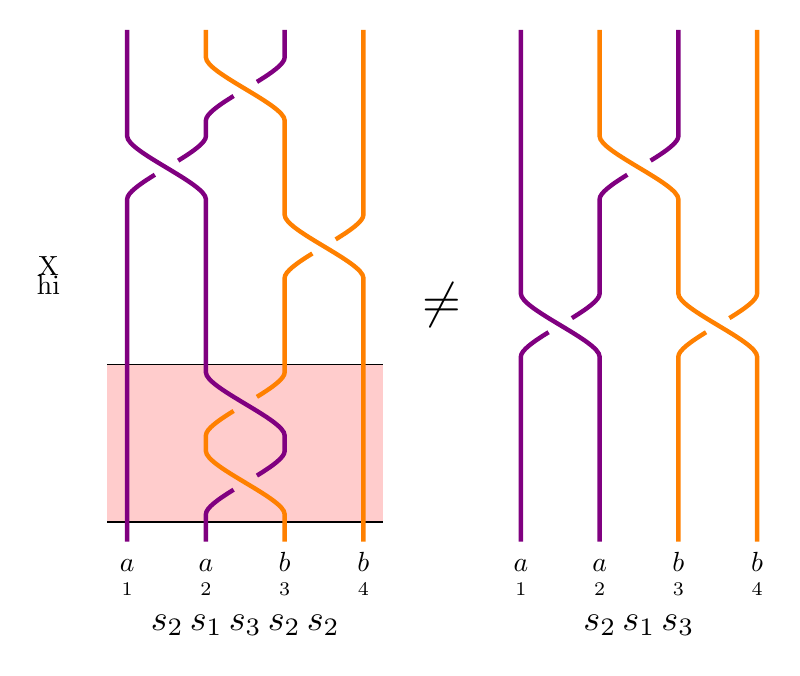
\begin{tikzpicture}
  \tikzset{
    strandstyles/.style = {
      braid/.cd,
      every strand/.style={ultra thick},
      strand 1/.style={violet},
      strand 2/.style={orange},
      strand 3/.style={violet},
      strand 4/.style={orange},
      % width=20mm, % currently makes braids collide
      gap=.1, % strictly between 0 and .5
      control factor=0.3, % default .5
      nudge factor=0.1, % default .05
    }
  }
  \pic[
  name prefix=braid1,
  strandstyles,
  add floor={1,4,3,2,twist},
  floor twist/.style={draw,fill=red!20!white},
  ] at (0,0) {braid={s_2 s_1 s_3 | 1 s_2 s_2}};
  
  \pic[
  name prefix=braid2,
  strandstyles,
  ] at (5,0) {braid={1 s_2 1 s_1-s_3 1 1}};
  \node (node3) at (-1,-3) {X};
  \node at (node3.south) {hi}; % test node works fine
  %\node at (braid1.south) {hi}; % error: No shape named `braid1' is known


  % braid1 labeling from bottom; is there a less confusing way?
  \foreach \x/\y/\z in {1/a/2,2/b/4,3/a/1,4/b/3}
  \draw
  (braid1-\x-e) ++(0,-.5ex) node[text height=.6cm] {$\y$}
  +(0,-3.5ex) node {$\scriptstyle \z$}
  ;
  % braid2 labeling from bottom
  \foreach \x/\y/\z in {1/a/2,2/b/4,3/a/1,4/b/3}
  \draw
  (braid2-\x-e) ++(0,-.5ex) node[text height=.6cm] {$\y$}
  +(0,-3.5ex) node {$\scriptstyle \z$}
  ;

  % there must be a better way to position these
  \draw
  ($(braid1-3-e)!.5!(braid1-2-e)$) ++(0,-7ex) node[scale=1.3]
  {$s_2 \, s_1 \, s_3 \, s_2 \, s_2$}
  %
  ($(braid2-3-e)!.5!(braid2-2-e)$) ++(0,-7ex) node[scale=1.3]
  {$s_2 \, s_1 \, s_3$}
  %
  (5,-3.5) ++(-1,0) node[scale=1.8]
  {$\not =$}
  ;
\end{tikzpicture}

\end{document}
